\documentclass[UTF8]{article}

\usepackage{CTEX}
\usepackage{epstopdf}
\usepackage{amsmath}
\usepackage{amsfonts}
\usepackage{amssymb}
\usepackage{multirow}
\usepackage{adjustbox}
\usepackage{float}
\usepackage{graphicx}

\begin{CJK}{UTF8}{song}
\title{基于加速度传感器的双人体感乒乓球游戏\\
数字逻辑设计实验报告}
\author{计44~~王子云~~2014010303\\
计44~~柯云劼~~2014012086
}
\end{CJK}
\date{ }

\begin{document}
\maketitle
\newpage
\tableofcontents 
\newpage
\section{实验简介}
% 柯
体感游戏是视觉与本体和动作控制的集合,为了达到视觉与运动相结合的目的,采用加速度传感器与VGA显示器相结合的方法,通过JY901传感器的运动来完成对游戏界面中的拍的控制,双方博弈模拟真实的乒乓球游戏。实验实现了开始界面、计分、自动难度调解与游戏结束等功能,最后通过下载验证,游戏获得了较好的互动性、参与性与沉浸感。
\section{总体设计思路}
% 王

\section{关键技术分析}
% 自己写自己的
\subsection{加速度传感器模块}
使用uart串口协议,一根数据输出线接入TX,一根数据读取线接入RX。
	\begin{figure}[H]
		\centering
		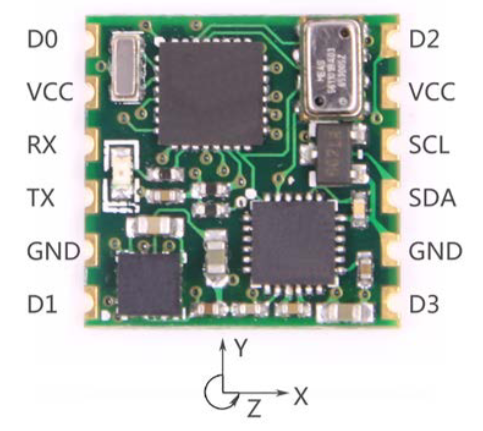
\includegraphics[width=2in]{2-1.png}
			\caption{JY901加速度传感器}	
	\end{figure}
\subsubsection{uart协议解析}
双方约定好时钟信号频率,波特率:115200(所以不像i2c或spi协议需要时钟线,但也造成了双方时钟可能会出现些偏差,导致会出现部分丢包现象)\par
获取由01电平组成的8字节长的数据包,双方统一约定电平拉低为8字节数据开始,电平拉高为8字节数据结束。\par
\subsubsection{传感器数据解析}
其中核心数据由16进制发送,也就是两个数据包组合为一个完整数据。默认第一个为低电平,第二个为高电平,需要将二者组合成一个有符号的short类型的数据。\par
多个数据组合为一个完整的输出,其中首项为设备地址,次项为输出地址,末项为校验和。\par
输出的具体解析公式方式如下:
	\begin{figure}[H]
		\centering
		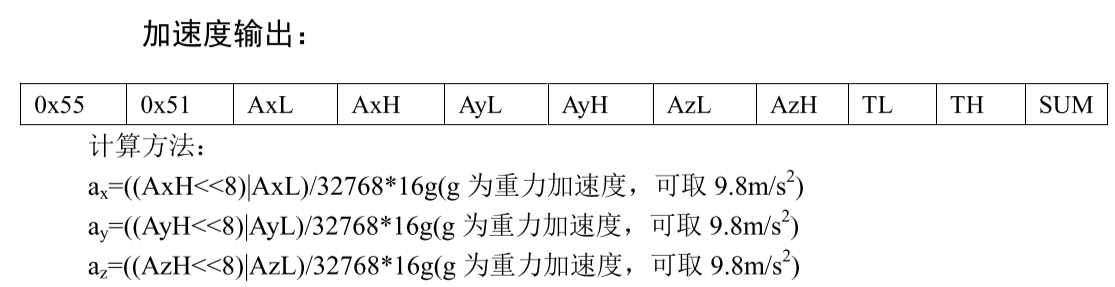
\includegraphics[width=\linewidth]{2-2.png}
			\caption{JY901加速度输出}	
	\end{figure}
	\begin{figure}[H]
		\centering
		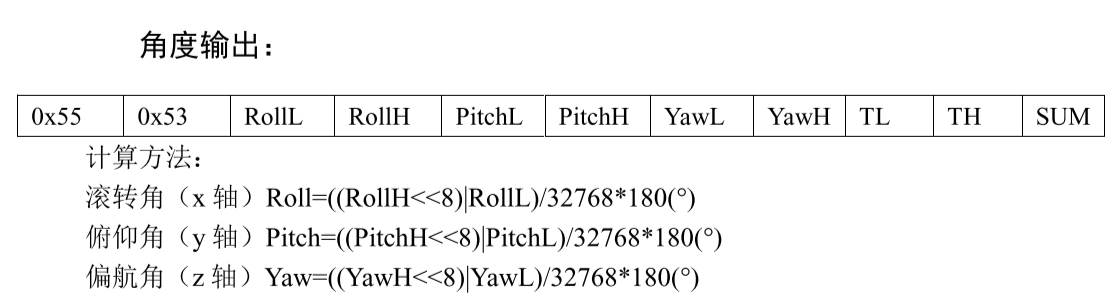
\includegraphics[width=\linewidth]{2-3.png}
			\caption{JY901姿态角输出}	
	\end{figure}
\section{下载验证及演示说明}
% 柯
\subsection{游戏中传感器操作方法}
初始预先设定将传感器片水平,将x轴方向指向前侧,y轴方向指向右侧。
\begin{enumerate}
\item 挥拍操作:传感器快速向前方击出
\item 移动拍操作:传感器绕x轴左右转动
\end{enumerate}
\subsection{游戏流程说明}
\begin{enumerate}
\item 游戏烧入至FPGA板上后,VGA显示器上显示开始界面。
\item 按RST建重置使游戏进入准备状态
\item 按键盘Enter,从开始界面进入游戏状态
\item 游戏预设先由屏幕左方发球。
\item 发球时球在与拍面夹角为$60^\circ-120^\circ$的区间内在拍面前来回转动。
\item 击出球后,球按着之前的轨迹在三维空间内运动。考虑到传感器操作比起实际运动的差异,故为了提供较好的用户体验,这里设置在左右边界处会发生碰撞使得游戏不会过早终止。
\item 当球进入另一方的击球区域后,若对方在球前方作出击球动作,则球被击回,挥拍力度将作为球的速度,进入6。
\item 若无法及时作出击球回应,则当球过了己方边界己方判负,对方获得一分,同时由对方发球,进入5。
\item 最先获得7分的一方获得本轮胜利,进入结束画面。
\item 按ESC可开始新一轮游戏,进入4。
\end{enumerate}
\section{实验中遇到的问题}
\subsection{传感器输出到游戏的物理运算}
\subsubsection{关于传感器的坐标变换}
之前设计中打算采用加速度进行二次积分出位置的方法:\par
传感器给出的加速度是以体轴坐标系作为参考的,\par
	\begin{figure}[H]
		\centering
		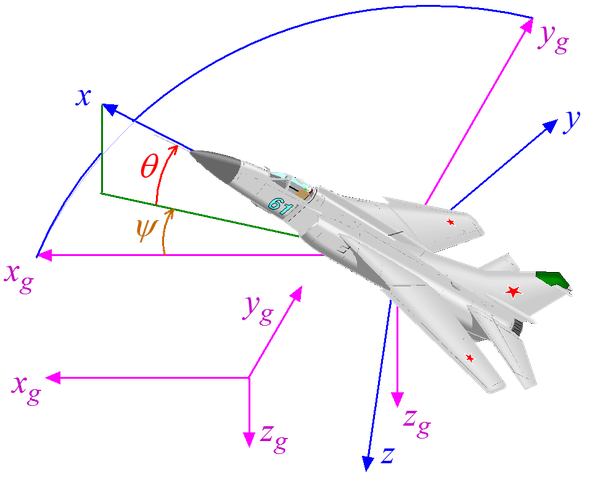
\includegraphics[width=3in]{2-4.png}
			\caption{体轴坐标系}	
	\end{figure}
故数据为了使用需要乘以一个体轴坐标系到地轴坐标系的变换矩阵。
这里介绍地轴坐标系到体轴坐标的变换,而所求变换即是原变换的逆操作。
原变换以先绕x轴旋转,再绕y轴旋转,最后绕z轴旋转进行。
	\begin{figure}[H]
		\centering
		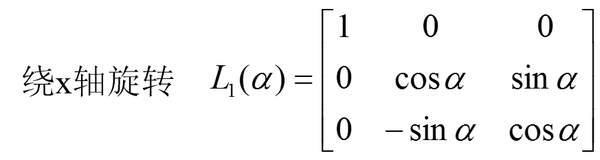
\includegraphics[width=3.5in]{2-5.png}
	\end{figure}
	\begin{figure}[H]
		\centering
		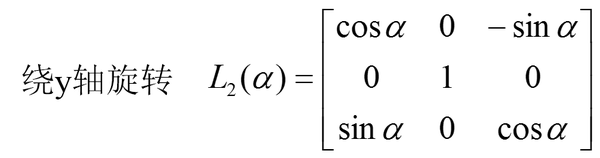
\includegraphics[width=3.5in]{2-6.png}
	\end{figure}
	\begin{figure}[H]
		\centering
		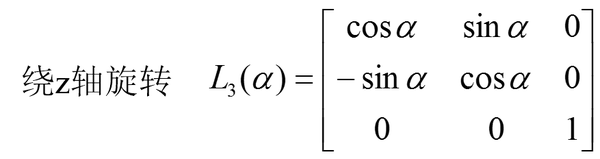
\includegraphics[width=3.5in]{2-7.png}
	\end{figure}
	\begin{figure}[H]
		\centering
		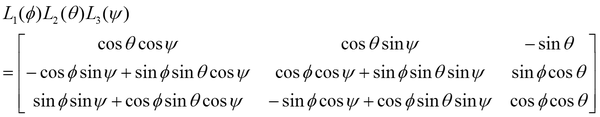
\includegraphics[width=\linewidth]{2-8.png}
			\caption{地轴坐标系到体轴坐标的变换矩阵}	
	\end{figure}
注意到该变换矩阵是正交矩阵,所求逆矩阵即为该矩阵的转置。
\subsection{三角函数的获得}
由于三角函数是浮点值,而FPGA中不支持浮点运算,考虑乘以1000来表示原三角函数值,在运算末尾再除以1000即可。\par
又由于FPGA没有简单的获得三角函数值得方法,经取舍后决定使用rom来读取。

\section{总结与体会}
% 王

\end{document}